\documentclass{article}
\usepackage{graphicx}
\usepackage{hyperref}
\usepackage{amsmath}
\usepackage[a4paper, total={6in, 8in}]{geometry}

\begin{document}

\begin{titlepage}
    \begin{center}
        \vspace*{1cm}
            
        \Huge
        \textbf{Electricity Usage Optimizer}
            
        \vspace{0.5cm}
        \LARGE
        Miniproject Report
        
        \date{today}
            
        \vspace{1.5cm}
            
        Pontus Hedlund, Sanna Korpi, Topi Ranta
            
        \vfill
            

            
        \vspace{0.8cm}
            
            
        \Large
        University of Helsinki\\
        Introduction to Data Science\\
        31.10.2022\\
            
    \end{center}
\end{titlepage}

\tableofcontents

\vspace{30.0 cm}

\section{A Simple Prediction of Electricity Price Development}
\label{section:introduction}

This report describes technical aspects of an electricity price prediction software made as Introduction to Data Science course mini project. The estimation tool is a Python web application that provides a 72-hour electricity price development prediction based on a model trained with \href{https://xgboost.ai/}{XGBoost library}. The forecast is shown as an hourly three-step recommendation scale and it is based on a linear regression model trained using historical data including electricity price, wind power, power consumption and weather data.

The report includes references to \href{https://github.com/IDS-mini/electricity}{the project repository in Github}. In addition to the data exploration, the regression model and the web application source code, the repository also includes our \href{https://github.com/IDS-mini/electricity/blob/main/marketing/Mini-Project-Canvas-Hedlund-Korpi-Ranta.pdf}{project canvas}, \href{https://github.com/IDS-mini/electricity/blob/main/marketing/presentation.pptx}{product pitch presentation} and \href{https://github.com/IDS-mini/electricity/blob/main/src/app/templates/index.html}{web application home page}. As this report does not discuss the added value or the business side of the project, it is advisable to walk through those documents before reading this technical report.

The rest of the report is composed as follows: the data used and data preprocessing are described in Chapter \ref{section:data}. The prediction formulation and the linear regression model used in the project are reported in Chapter \ref{section:analysis}. User experience and results delivery for the end user are displayed in Chapter \ref{section:delivery}. Observations, discussion and ideas for further development are presented in \ref{section:conclusions}.

\section{Data}
\label{section:data}

In order to produce the prediction, several sets of historical data were used. The data sets are described in Subchapter \ref{subsection:datadescription} and comments on the data exploration and preprocessing in Subchapter \ref{subsection:eda}. Data storage and protection are reported in Subchapter \ref{subsection:warehousing}.

\subsection{Data Used in the Project}
\label{subsection:datadescription}

%% why this data, ref to feature extraction

The data sources used in the project are \href{https://data.fingrid.fi/en}{Fingrid Wind Power Production and Total Consumption Data}, \href{https://transparency.entsoe.eu}{Entsoe Day-ahead Market Price Data}, \href{https://en.ilmatieteenlaitos.fi/open-data}{Finnish Meteorological Institute Weather Observation Data for Kumpula, Helsinki}. The data was accessed in two ways. Large, historical data sets were manually downloaded for exploration, feature extraction and model training and programmatic access was used to enable the web application to get the latest data for user predictions. The programmatic access includes API connections and web scraping.

Even though all the data is available for free, some sources require registering an account to download the full data or access most recent data via API. Characteristics of the data sources are presented in Table \ref{table:source-characteristics}.

\begin{table}[ht] 
\centering 
\begin{tabular}{l||l c c} 
data set & Format & Access via & Registration\\ 
\hline \hline
Entsoe & CSV & UIM, WS  & Required for full history access \\
FMI & CSV & UI, API & Not required \\
Fingrid & CSV & UIM, API & Required for API access \\
\hline
\end{tabular}
\caption{The data sources used in the project. UIM is abbreviation for manual download via user interface and WS for web scraping.}
\label{table:source-characteristics}
\end{table}

Entsoe Day-ahead Prices data consists of hourly electricity market prices for Finnish Bidding Zone that covers the whole country. \href{https://data.fingrid.fi/en/data set/wind-power-generation}{The Wind Power Production} data set includes hourly wind power production in Finland in $MWh/h$, \href{https://data.fingrid.fi/en/data set/electricity-consumption-in-finland}{Electricity Consumption} data set $MWh/h$ consumption and from \href{https://en.ilmatieteenlaitos.fi/open-data}{Weather Data} we picked air pressure, rain, humidity, temperature and wind. \href{https://www.helen.fi/en/company/responsibility/current-topics/open-data}{Helen District Heating Power Data} was investigated but was reject, as the data was only available until the end of year 2021.

All the data used in project is provided in one hour interval thus making data integration rather easy. The historical data was downloaded spanning from the beginning of 2019 as far ahead as possible. Beginning of 2019 was chosen so that the current volatile prices would not be marginalized in the data set. A visualization of 2022 price volatility can be viewed in Figure \ref{fig:prices-history}.

\begin{figure}[ht] 
\centering
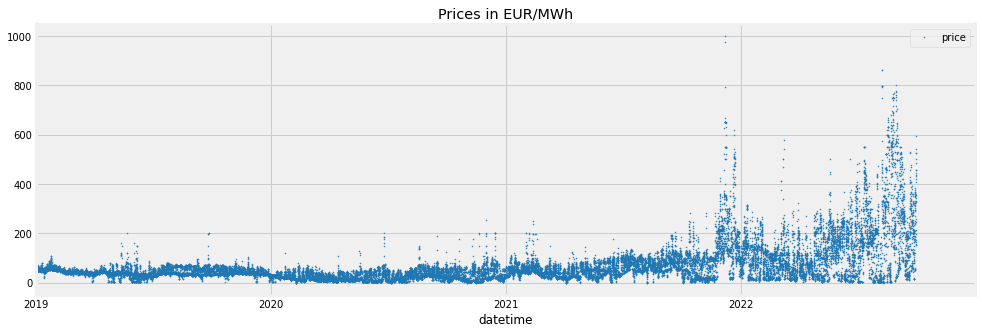
\includegraphics[width=\textwidth]{report/images/day-ahead-prices.png}
\caption{Day-ahead market prices for electricity in Finland.}
\label{fig:prices-history} 
\end{figure}

\subsection{Exploratory Data Analysis and Data Preprocessing}
\label{subsection:eda}

The purpose of the exploratory data analysis (EDA) and data preprocessing phase was to understand the data and its possible shortages and produce an integrated data set for model training with missing values imputed. This phase was conducted in series of Jupyter Notebook files. The cleaned csv files were written into Apache Parquet format for better data compression and reading performance before integration. The eda and data cleaning notebooks are listed in Table \ref{table:eda}.

As expected, the data cleaning and integration was rather effortless. Missing data rates were low (for example, less than 0.4\% day-ahead prices were missing) and missing values imputation was performed using neighbor values, which intuitively works well with time-series data. In the cleaning process, datetime column was set as data set as index and was thus later used as key to integrate the cleaned parquet files.

\begin{table}[ht] 
\centering 
\begin{tabular}{l||l c} 
Data set & Imputation method & File\\ 
\hline \hline
Day-ahead & Previous neighbor & \href{https://github.com/IDS-mini/electricity/blob/main/data/day-ahead_clean.ipynb}{day-ahead\_clean.ipynb},  \href{https://github.com/IDS-mini/electricity/blob/main/data/day-ahead_eda.ipynb}{day-ahead\_eda.ipynb}\\
Consumption & - & \href{https://github.com/IDS-mini/electricity/blob/main/data/consumption_eda.ipynb}{consumption\_eda.ipynb} \\
Weather & Neighbor values mean & \href{https://github.com/IDS-mini/electricity/blob/main/data/weather_eda.ipynb}{weather\_eda.ipynb} \\
Wind power & - & \href{https://github.com/IDS-mini/electricity/blob/main/data/wind_power_eda.ipynb}{wind\_power\_eda.ipynb}\\
\hline
\end{tabular}
\caption{The data sets used to train the model. Links to data sets' EDA Jupyter notebook files are presented in the File column.}
\label{table:eda}
\end{table}

In addition to the cleaned historical data, time series forecasts for each data sets were created. The former were used to train the model and the latter, supplemented with latest data renewed via programmatic data fetching, to construct final predicted price. The data was integrated in \href{https://github.com/IDS-mini/electricity/blob/main/data/data_integration.ipynb}{data\_integration.ipynb} where new features were also extracted. Both feature extraction and prediction creation process are further discussed in Chapter \ref{section:analysis}.

%% eda findings

    %% week and day cycle of electricity price
    %% cold weather effecting consumption
    %% connection between consumption and price

\subsection{Data Warehousing and Data Protection}
\label{subsection:warehousing}

Both the raw, manually downloaded data and the cleaned data were stored in the project repository. As datasets were reasonably-sized, data files being around 0.5 MB, we evaluated the code repository solution to be adequate. Larger project would have required a more scalable warehousing solution, for example a cloud-based blob storage.

All data used in our project is publicly available and does not include any personal data, so no data used in the project was subject to the GDPR act. Therefore, the warehousing solution's sole purpose was to share the data changes and cleanings between project developers and to keep the data backed up and version controlled.

\section{Data Analysis}
\label{section:analysis}

The purpose of the project and the data analysis was to create a 72-hour estimate on electricity hourly market price development. In order to do so, we extracted new features from the cleansed and integrated data, wrote scripts for refreshing the data and supplementary predictions. The feature extraction is reported in Subchapter \ref{subsection:extraction}, training the XGBoost Regressor is presented in Subchapter \ref{subsection:xgboost} and data refreshing and intermediate forecasts to support contemporary predictions are discussed in Subchapter \ref{subsection:datafilling} .

\subsection{Feature Extraction}
\label{subsection:extraction}

%% time series features

First, we extracted new features from datetime index itself. As electricity usage and thus market price fluctuations are cyclic and depend on time of the year, weekday, time of the day and so on, the datetime was decomposed to several new features. A rather intuitive example of how we thought these features might affect the rest of the data components is illustrated in Figure \ref{fig:components}.

\begin{figure}[ht] 
\centering
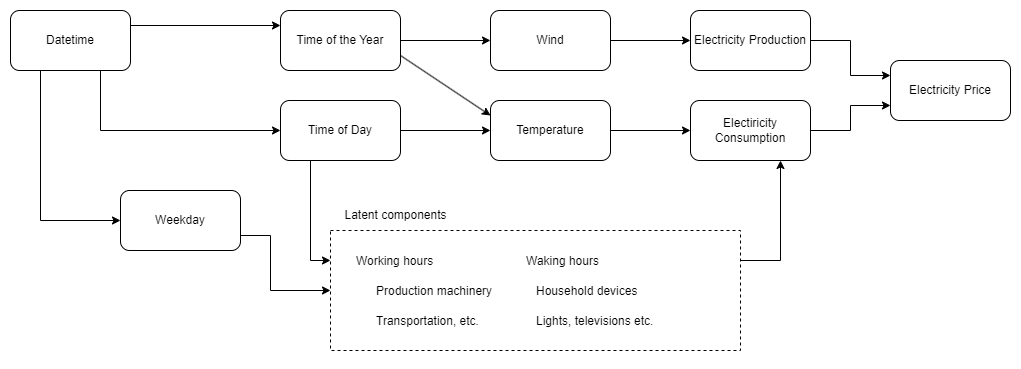
\includegraphics[width=\textwidth]{report/images/components.png}
\caption{A simplified diagram on how we assumed different components could affect each other and thus the target value.}
\label{fig:components} 
\end{figure}

Second, lag features were extracted from the data. The data was supplemented with component values from one, two and three years ago. %% why these

\subsection{Time Series Prediction with XGBoost}
\label{subsection:xgboost}

After feature extraction, the features chosen to eventually train the model were \textbf{Consumption, Wind, Air Pressure, Rain, Humidity, Temperature} and \textbf{Wind} with their three corresponding lag features. In addition, \textbf{Day of Year, Hour, Day of Week, Quarter, Month} and \textbf{Price lag features} were added to the features. The Price itself as it was set as target value.

The machine learning model used for this application is the XGBoost Regressor, which is an ensemble method based on gradient-boosted decision trees. We found it to be very fast to train and very accurate. In addition we had some experience on XGBoost from previous projects. 

When training the models, we used cross-validation with time series splits so that we could validate the model with real past data. An illustration of cross-validation can be seen in Appendix A, Figure \ref{fig:ts-cross-validation}.



\subsection{Gathering the Data for the Prediction}
\label{subsection:datafilling}

As the model is trained on past data, all the same variables need to be present when performing the contemporary prediction. Not all of these are available for each prediction time. For example, for obvious reasons, we do not have historical data for humidity 24 hours in the future.

To circumvent the problem, we created time series forecasts as a base that should give a best estimate of the values. An example of Consumption forecast is presented in Figure \ref{fig:consumption} in Appendix \ref{section:appendixa}. Also, Finnish Meteorological Institute's two-day forecast is exploited when filling the future data. This forecasted base is then updated with programmatic data fetching as data is available from data sources.

The forecast is part of the web application's code. In addition, the prediction is automatically run twice a day with Github actions and saved to the repository. The web application then tries to use this prepared data when showing the recommendations for the end user. Deriving the recommendation from the forecasted price is discussed in more detail in Chapter \ref{section:delivery}. 

\begin{figure}
    \centering
    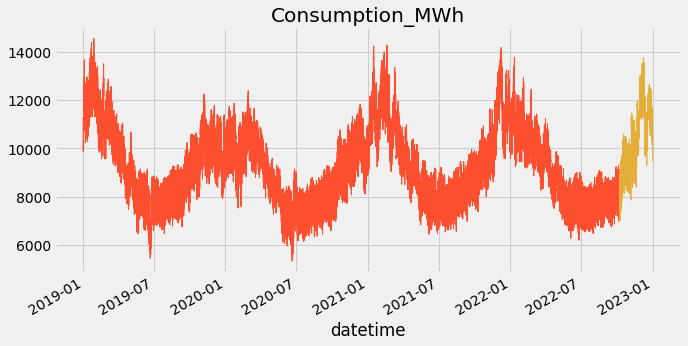
\includegraphics[width=15cm]{report/images/consumption.png}
    \caption{Time series for Consumption in MWh with historical data in red and the forecast in orange.}
    \label{fig:consumption}
\end{figure}


\section{Delivering Results for the End User}
\label{section:delivery}

For the contemporary results delivery to the end user, we built a simple Python web application. To make the prediction more comprehensible for the end user, a three-level recommendation is inferred from the predicted price. The web application with invoking instructions is briefly presented in Subchapter \ref{subsection:server} and the recommendation for the end user is described in Subchapter \ref{subsection:ux}.

\subsection{Web Application}
\label{subsection:server}

Our deliverable is a web application built with FastAPI. The application serves a landing page and a page for planning. The landing page includes some instructions and reasons for electricity usage optimization and plan page shows a table with hourly times for the next 72 hours with a recommendation and the price index. The whole package is available on Github at https://github.com/IDS-mini/electricity.

To run the app, one needs API key for the \href{https://data.fingrid.fi/open-data-forms/registration/}{Fingrid API} which is set into an environment variable used by \href{https://github.com/IDS-mini/electricity/blob/main/src/app/utils/fetch_consumption.py}{fetch\_consumption.py}. The project authors' API key is not stored in the public repository. For project evaluation purposes the API key can be acquired from the project authors via their university email addresses. Since the web application is fairly simple, comprehensive user interface screenshots are provided in Appendix \ref{section:appendixb} and current predictions may be viewed in the \href{https://github.com/IDS-mini/electricity/blob/main/forecast_data/forecasts.csv}{project repository}.

\subsection{Electricity Usage Recommendation and User Experience}
\label{subsection:ux}

As the market price is currently extremely volatile, we wanted to avoid obvious prediction pitfalls. A precise, hourly $EUR/kWh$ prediction could be easily perceived faulty if it would not hit the target accurately. Furthermore, it would not convey the right message as we wanted to assist the end user to find the cheapest and most expensive periods of time in the near future rather than predict the sum of their next electricity bill.

Therefore, instead of a monetary value per hour, we created a three-step scale to steer the end user: \textbf{boost}, \textbf{maintain} or \textbf{restrict} electricity usage. To achieve this, we calculate a simple moving average (SMA) of the electricity price with a window of last 168 hours (7 days) to create a reference price point. For each prediction time, we compare the predicted or known price to the index. The calculation is illustrated in Equation \ref{eq:index}.


\begin{equation} \label{eq:index}
\text{"Price Index"}_i = \frac{\text{SMA}_i}{\text{"Predicted Price"}_i}
\end{equation}

The price index is then classified as follows:

\begin{enumerate}
    \item $\text{"Price Index"}_i < 0.8$ : "Boost"
    \item $0.8 \leq \text{"Price Index"}_i \leq 1.2$ : "Maintain"
    \item $\text{"Price Index"}_i > 1.2$ : "Restrict"
\end{enumerate}

The steps are then color coded to green, yellow and red so that user can easily spot the coming peaks. As the prediction is fully based on public data, the web application does not collect data from the end user.

\section{Discussion and Conclusions}
\label{section:conclusions}

In this report we have presented how data was gathered and preprocessed, how machine learning model was trained, how supplementary predictions were made and how a comprehensible prediction for the end user was derived to assist the end user to optimize their electricity usage. 

%% what was achieved
%% what was learned
%% what we would do differently
%% ideas for further development or research


\appendix
\section{Data Illustrations}
\begin{figure}
    \centering
    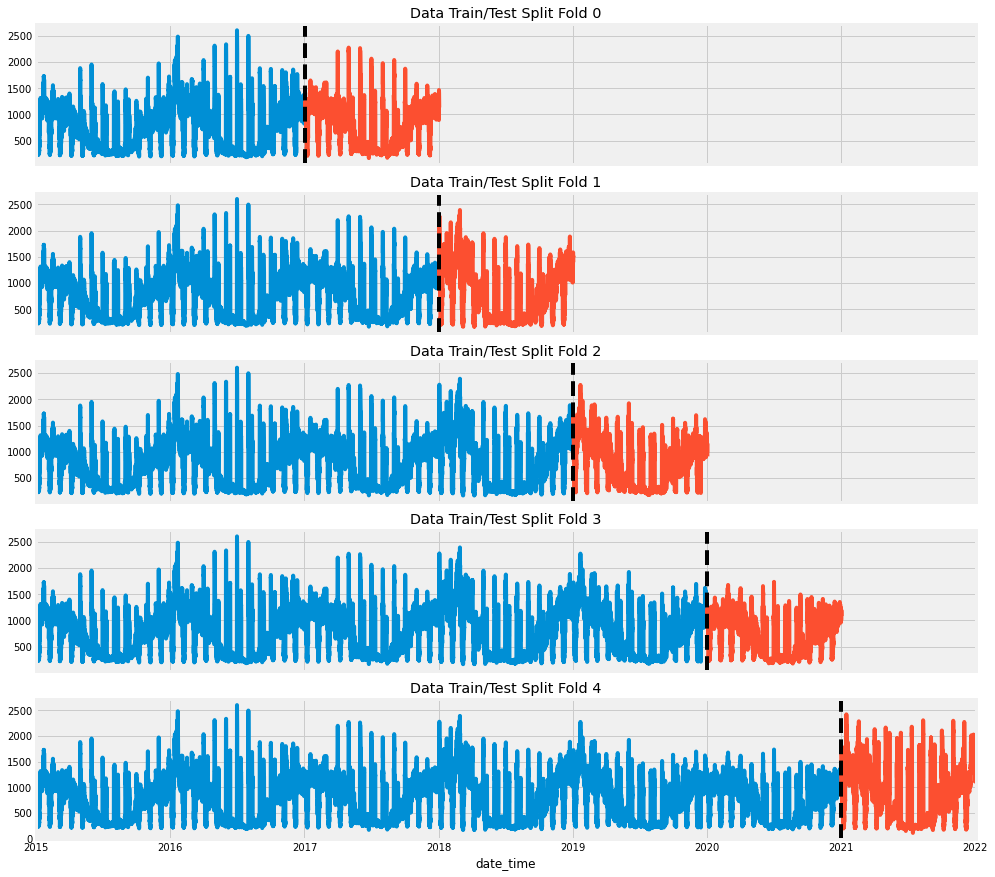
\includegraphics[width=15cm]{report/images/ts-cross-validation.png}
    \caption{Cross validation using Time Series Splits with each split being a year.}
    \label{fig:ts-cross-validation}
\end{figure}
\label{section:appendixa}

\section{Application User Interface Screenshots}
\begin{figure}[H]
    \centering
    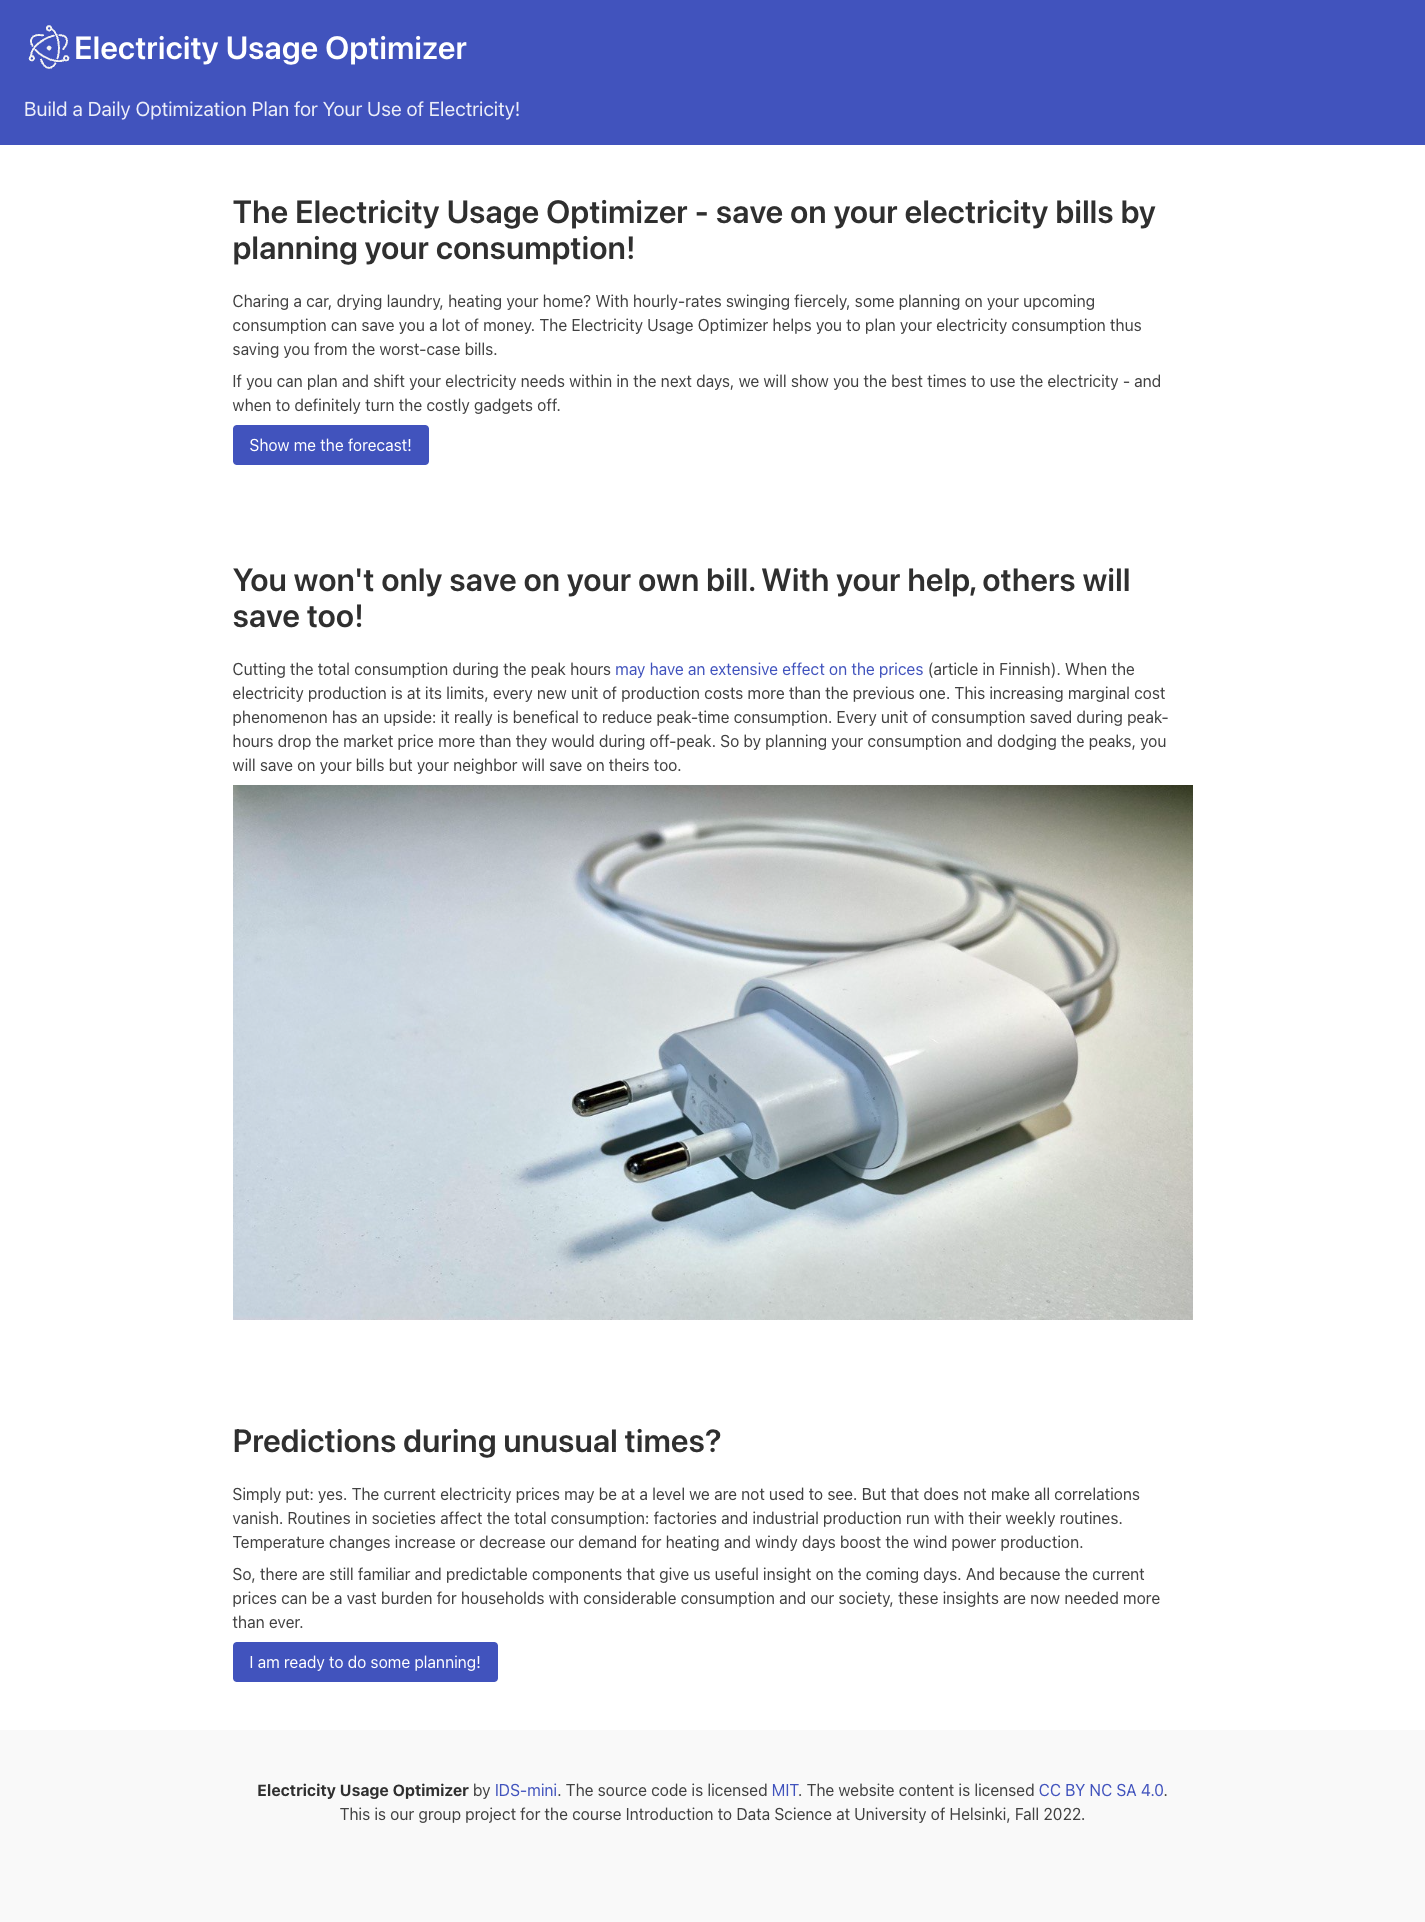
\includegraphics[height=0.9\textheight]{report/images/application-home-page.png}
    \caption{Application home page.}
    \label{fig:app-home-page}
\end{figure}

\begin{figure}[H]
    \centering
    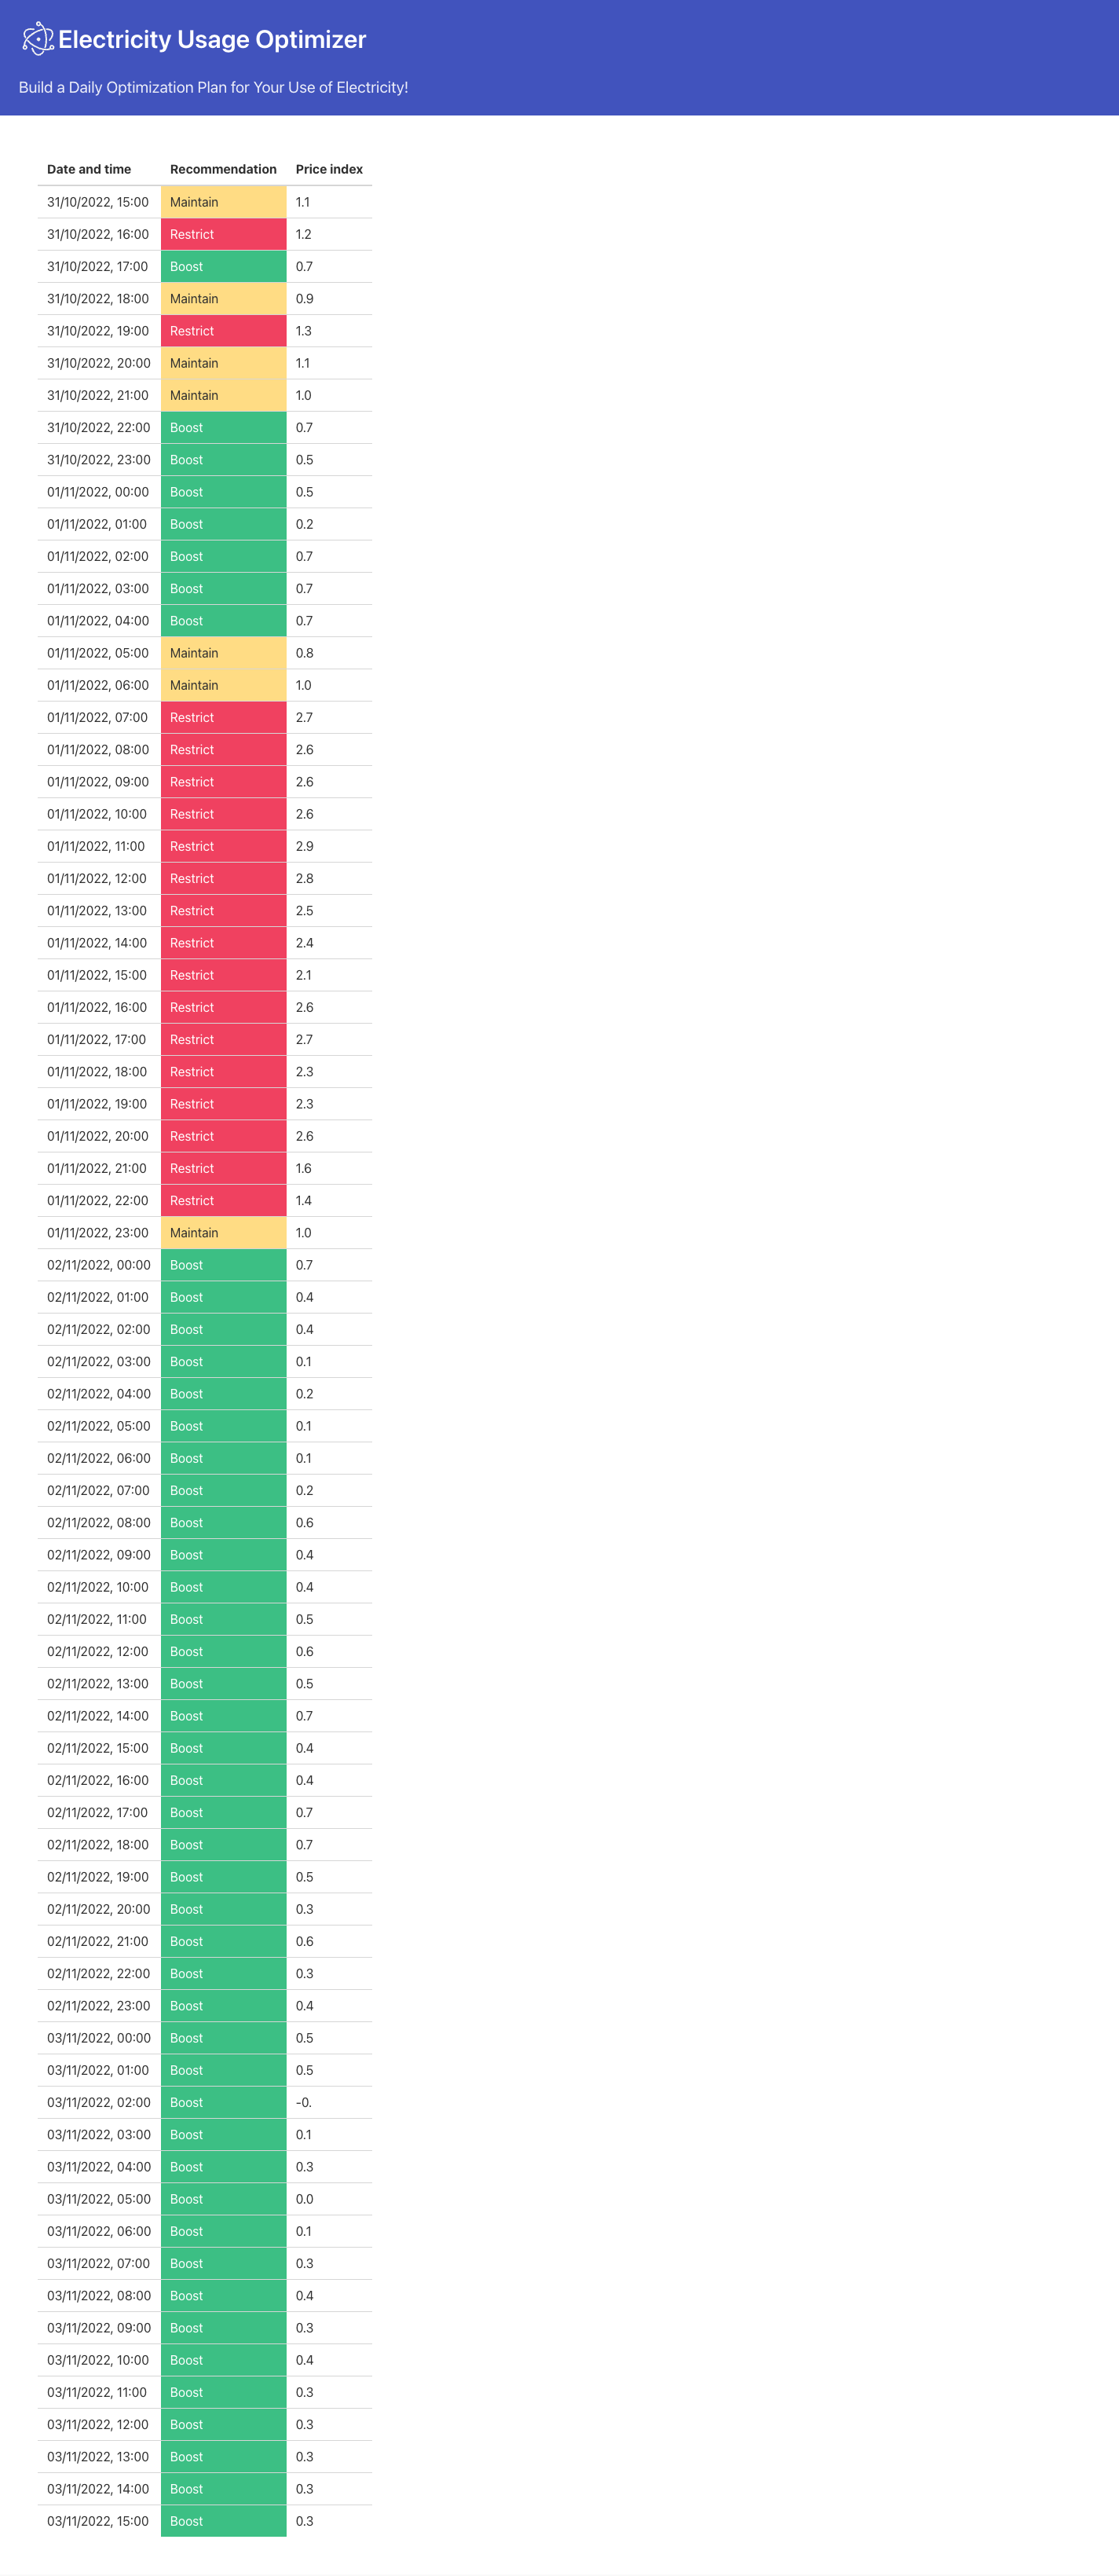
\includegraphics[height=0.9\textheight]{report/images/application-planning.png}
    \caption{Application planning page. The first 24 hours of prediction have been replaced with available day-ahead market price. The day-ahead prices tend to be somewhat higher than our prediction, which in this case makes the rest of the 72-hour period appear relatively cheap.}
    \label{fig:app-planning-page}
\end{figure}
\label{section:appendixb}


\end{document}

